
%%% Local Variables:
%%% mode: latex
%%% TeX-master: t
%%% End:

\chapter{资源管理软件栈研究}
\label{chap:prm}

实现高效资源管理需要软硬件协同设计。
PARD体系结构已经实现将硬件资源信息暴露给上层软件,
并提供可编程接口给软件访问,本章主要讨论在PARD这样的硬件架构平台上,
如何实现设计软件栈以实现高效的资源管理。
则一般都会影响甚至重构整个软件栈:最底层的控制平面驱动层,负责直接访问控制平面,这一层可以部署在操作系统、Hypervisor或者一个轻量级的操作系统内核;在驱动层上面为监控管理层,主要负责集中存储收集到的各个控制平面的统计数据,并将多个控制平面关联分析,进行资源分配管理的决策;更上层是用户编程接口层,主要负责提供对控制平面统一的抽象编程接口以及对统一、决策功能的抽象编程接口;最上层则是数据中心管理软件层,主要负责收集几个计算机节点的资源信息,进行全局作业调度与资源管理,以实现在保障关键应用服务质量的前提下达到全局资源利用率最优化。
因此,从单个计算机节点角度出发,在硬件支持资源管理的基础上,软件栈的设计与实现需要研究上述驱动层、监控管理层与用户接口层的设计与实现,降低软件栈的设计复杂度与运行开销,研究针对不同资源的优化管理策略。同时研究在这种新体系结构下对软件虚拟化技术的影响。

PARD体系结构在硬件上有两方面的改变:一是一部分资源管理功能放到了硬件控制器上;二是将更多的硬件资源信息暴露给软件。计算机底层硬件功能的改变会对上层软件栈产生影响。

\section{背景}

PARD软件栈负责管理节点内的硬件资源,同时需要与数据中心管理软件交互,
实现数据中心范围内的全局资源管理。
为了实现XXX,PARD的软件栈运行在独立的硬件部件上,与IPMI类似,
本节首先介绍IPMI\cite{ipmi}与带外管理相同的背景,
然后介绍Mesos\cite{Hindman:2011:Mesos}的架构。

介绍IPMI/BMC与带外管理,PARD的软件栈在此基础上进行扩充。

mesos/openstack做为数据中心OS,其架构,PARD要接入到这些架构中。


\subsection{带外管理与IPMI}

In computing, one form of out-of-band management is sometimes called lights-out management (or LOM) and involves the use of a dedicated management channel for device maintenance. It allows a system administrator to monitor and manage servers and other network-attached equipment by remote control regardless of whether the machine is powered on, or if an operating system is installed or functional.

By contrast, in-band management like VNC or SSH is based on in-band connectivity and software that must be installed on the remote system being managed and only works after the operating system has been booted. This solution may be cheaper, but in computing it does not allow access to firmware (BIOS or UEFI) settings, does not make it possible to reinstall the operating system remotely, and it cannot be used to fix problems that prevent the system from booting. In networking, it does not allow management of remote network components independently of the current status of other network components.

Both in-band and out-of-band (OOB) management are usually done through a network connection, but an out-of-band management card can use a physically separated network connector if preferred. A remote management card usually has at least partially independent power supply, and can power the main machine on and off through the network.

The Intelligent Platform Management Interface (IPMI) is a set of computer interface specifications for an autonomous computer subsystem that provides management and monitoring capabilities independently of the host system's CPU, firmware (BIOS or UEFI) and operating system. IPMI defines a set of interfaces used by system administrators for out-of-band management of computer systems and monitoring of their operation. For example, IPMI provides a way to manage a computer that may be powered off or otherwise unresponsive by using a network connection to the hardware rather than to an operating system or login shell

\begin{figure}[tbh]
  \centering
  \includegraphics[width=0.95\textwidth]{swstk/ipmi-schem}
  \caption{IPMI结构框图}
  \label{fig:ipmi-schem}
\end{figure}

IPMI的结构如图\ref{fig:ipmi-schem}所示,其中主要包含以下几个模块:

\textbf{Baseboard Management Controller (BMC)}\quad
A micro-controller (BMC) is the heart of the IPMI architecture. The tasks of the BMC includes:
interfacing between the system management software and the hardware being used (through which the BMC has been connected using IPMB and ICMB)
monitoring independently
logging events independently
controlling recovery

\textbf{Intelligent Platform Management Bus (IPMB)}\quad
IPMI allows for the extension of the BMC by additional Management Controllers (MCs) through the application of the IPMB standard.
IPMB is an I²C based serial bus, which makes connection with various boards inside of one chassis possible. It is used for communication to and between the management controllers (MCs). Additional MCs are often designated Satellite Controllers.

\textbf{Intelligent Chassis Management Bus (ICMB)}\quad
ICMB provides a standardized interface for communication and control between chasses.


\subsection{数据中心管理系统}

\begin{figure}[tbh]
  \centering
  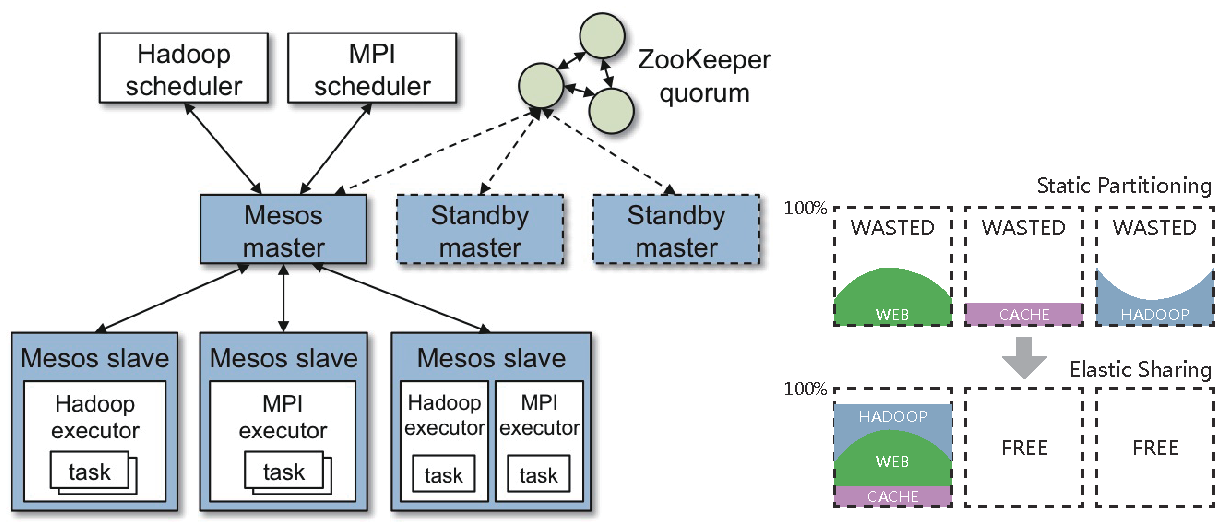
\includegraphics[width=0.7\textwidth]{swstk/mesos-arch}
  \caption{Mesos系统架构}
  \label{fig:mesos-arch}
\end{figure}

The above figure shows the main components of Mesos. Mesos consists of a master daemon that manages slave daemons running on each cluster node, and Mesos frameworks that run tasks on these slaves.

The master enables fine-grained sharing of resources (CPU, RAM, …) across frameworks by making them resource offers. Each resource offer contains a list of <slave ID, resource1: amount1, resource2, amount2, …>. The master decides how many resources to offer to each framework according to a given organizational policy, such as fair sharing or strict priority. To support a diverse set of policies, the master employs a modular architecture that makes it easy to add new allocation modules via a plugin mechanism.

A framework running on top of Mesos consists of two components: a scheduler that registers with the master to be offered resources, and an executor process that is launched on slave nodes to run the framework’s tasks (see the App/Framework development guide for more details about framework schedulers and executors). While the master determines how many resources are offered to each framework, the frameworks' schedulers select which of the offered resources to use. When a frameworks accepts offered resources, it passes to Mesos a description of the tasks it wants to run on them. In turn, Mesos launches the tasks on the corresponding slaves.

\section{软件栈平台与架构}

基于IPMI,增加控制平面网络,实现与控制平面通信

\begin{figure}[tbh]
  \centering
  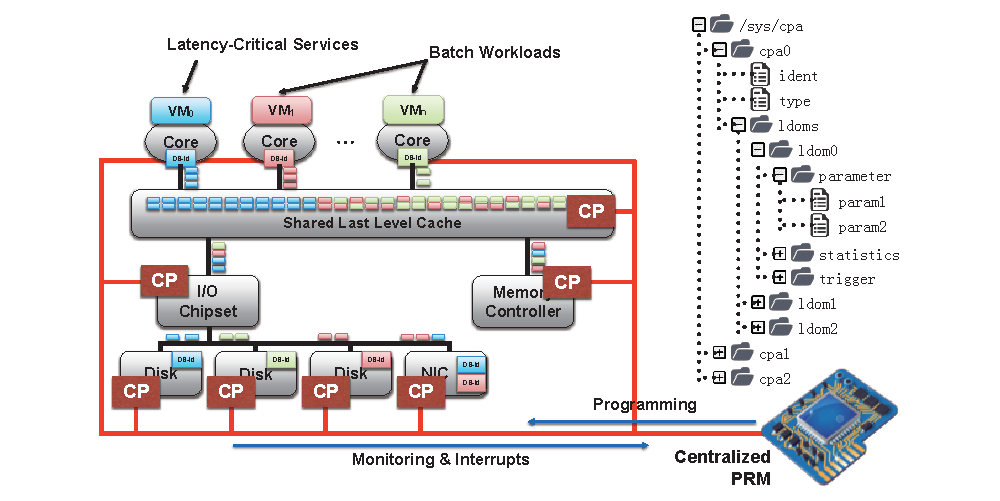
\includegraphics{arch/pard-arch-outline.pdf}
  \caption[PARD体系结构概况]{PARD体系结构概况}
  \label{fig:pard-arch-outline}
\end{figure}


Like IPMI [6] in conventional servers, PARD includes a
per-computer centralized platform resource manager (PRM) that
connects all control planes and tag registers (see the dash lines in
Figure 2). PRM is essentially an embedded system-on-chip (SoC)
that consists of an embedded processor, RAM, flash, a local bus, an
Ethernet adaptor and several control plane adaptors (CPAs).

A Linux-based firmware running on PRM abstracts all control
planes as a device file tree that is logically centralized. The
firmware provides a uniform file based programming interface to
access different control planes and a more advanced “trigger)action”
programming methodology (see below) for operators to create and
deploy resource management policies.


\section{节点内资源管理}

\subsection{控制平面抽象}

将控制平面抽象为文件,实现软件编程

To provide a uniform interface for firmware users (data center operators)
to access various control planes, we leverage Linux’s device
file mechanism. Figure 6 shows the abstraction of the control planes
from a firmware user’s perspective. Specifically, each control plane
is connected to a PRM’s control plane adaptor (CPA) that is abstracted
as a file and is mounted to the sysfs [55] of the firmware as
“/sys/cpa/cpa[0-9][0-9]*”. Thus firmware users can use either bash
commands (e.g., cat or echo) or system calls to access these files.
Each control plane file is organized as a subtree, which contains
some general information such as ident (e.g., cpa0’s “CACHE CP”
in Figure 6) and type indicating which type of a control plane
is, cache (“C”), memory (“M”) or I/O bridge (“B”). Besides, a
control plane file further includes several subtrees, each of which
represents a LDom with a specific DS-id. When a new LDom is
created, the firmware creates a new subtree with root “ldom[0-9][0-
9]*” under the node ldoms, where the number represent a DS-id.
Take the ldom0 subtree as an example, there are three tiny trees
with roots as parameters, statistics and triggers respectively, which
are mapped to several rows of the three tables of the LLC control
plane.

Programming Methodology
As mentioned in x3, we adopt a “trigger)action” programming
methodology. Data center operators predefine a set of trigger)action
rules for different priorities. Usually a trigger is based on performance
metrics, e.g., “MissRate>30%”.
Example 1 in Figure 6 demonstrates how to install a trigger)action
rule. A data center operator uses the pardtrigger command to program
the trigger condition “MissRate>30%” for “ldom=0” (i.e.,
DS-id=0) into the trigger table of the cache control plane (cpa0).
The parameter “action=0” guides the command to create a leaf
node “0” under “.../cpa0/ldoms/ldom0/triggers”. Then the operator
calls “echo ...” to install the action script “/cpa0 ldom0 t0.sh”
shown in Example 2.
There are two programming approaches based on the device file
tree. One is invoking system calls (open/read/write etc.) to open
and manipulate a CPA file. For example, the pardtrigger command
is written in C and invokes syscalls to install a trigger into the
cache control plane. The advantage of this approach is very fast. A
more convenient approach is leveraging bash commands to directly
access these CPA files, as shown in Example 2.


\subsection{实现虚拟机}


\subsection{实现QoS管理}


\section{与数据中心结合}



\section{小结}


应用负载具有波动性,对硬件资源的需求会发生变化,需要提供一种动态调整应用资源分配的方案。

有三个层次,分别:
(1)节点内不同硬件资源的协同管理;
(2)节点内应用调度与资源协同管理;
(3)节点间协同管理;


PRM软件接口,

- 与mesos集成,实现硬件支持的容器

- 与OpenStack集成,实现IaaS平台

- 与SDN集成,实现网络中心的系统

